\section{A Penalised Likelihood Approach to Joint Quantiles}\label{sec:obj_to_joint_estim}
%
\subsection{Notation}
%
The symbol $\sim$ is used both as a sampling statement as well as signifying a variable's probability density function or a likelihood function, synonymously written as $p\left(\right)$. This makes the notation close to probabilistic programming languages such as Stan \citep{carpenter_stan_2017}. Denote by $\mathcal{S}$ a non-empty sample space on which the $\sigma$-algebra $\mathcal{M}$ is defined. Then, by $P\left(X|Y\right)$ we denote the probability of $X=x$ given $Y=y$, where $(X,Y) \subseteq D$. We suppress the differentiation between random and ordinary bound variables for readability. We refer to all unspecified parameters in definitions of conditional probability density functions by $\vartheta$. 
%
\subsection{Motivation}\label{sec:motivation}
%
Let $X = (X_1,\dotsc,X_K)^T$ be a set of covariates which are related to a response vector $y$. Let $D \subseteq \mathbbm{R}^K$ be a closed convex polytope represented as the convex hull of $\mathcal{T}$~points in $K$~dimensions. We are interested in a regression at $\mathcal{Q}$~quantile levels $0<\tau_1<\dotsc<\tau_{\mathcal{Q}}<1$, where $\mathcal{Q}$ is a finite integer. Denote by $Q_{\tau_q}(X,\beta_q)$ the $q$\textsuperscript{th} quantile of $y$ as a function of $X$, given some set of quantile-specific regression coefficients $\beta_q$, such that $P\left(y\leq Q_{\tau_q}(X,\beta_q) \vert X, \beta_q \right) = \tau_q$. The classic solution to quantile function estimation approach is to presume quantile functions to be independent, regardless of $\mathcal{Q}$. However, this neglects that the quantile coefficients, $\beta_q$, are often correlated across  quantiles. Such information sharing can drastically improve inference, even if the modeller is only interested in inference on a single quantile \citep{bondell2010noncrossing,jiang2013interquantile}. The key interest in this paper, is to implement information sharing across  quantiles via priors on the differences of the quantile coefficients. Importantly, the quantile coefficient process is centred on a quantile invariant coefficient vector - akin to the composite quantile model \citep{zou2008composite}. By doing so, as differences are adaptively shrunk to zero, the model reduces to the composite quantile regression model, which estimates parallel quantile functions. In this way the model penalises quantile crossing.
%

To motivate the functional form of the prior, consider the following objective function: 
%
\begin{IEEEeqnarray}{rl}\label{eq:general-objective-function}
    \sum_{q=1}^{\mathcal{Q}}\sum_{t=1}^{\mathcal{T}} \rho_{\tau_q} & \left( y_t - \alpha_q - x_t^T\beta_0 - x_t^T\beta_q\right) + \mathrm{pen}\left( \left\{\beta_q\right\}_{q=1}^{\mathcal{Q}}\right)  
    \\
    \mathrm{s.t.}~ & x_t^T\beta_q + \alpha_q \geq x_t^T\beta_{q-1} + \alpha_{q-1} \; \forall q = 2,\dotsc,\mathcal{Q}, t = 1,\dotsc,\; \mathcal{T}, \label{eq:NC-constraint-facevalue}
\end{IEEEeqnarray}
%
where $\rho_{\tau_q}(u) = u(\tau_{q}-I(u<0))$ is the tick-loss function and the constraint in Equation~\ref{eq:NC-constraint-facevalue} ensures monotonicity of the conditional quantile functions. Here, $\alpha_q\in \mathbbm{R}$ is an intercept specific to each quantile. $\beta_0 \in \mathbbm{R}^{K}$ are the quantile invariant coefficients, and $\beta_q \in \mathbbm{R}^{K}$ capture the variation in the effects of covariates across quantiles. Denote by $x_t$ the $t$-th row of X. If $\alpha$ is a monotone function of $\tau$, then the penalty term included, shrinks the model to uniformly parallel, or pair-wise parallel lines. \citet{szendrei2023fused} show that when recasting the data domain to $x_t \in \left[-1,1\right]^{K}$,\footnote{Recasting the data domain to $x_t \in \left[-1,1\right]^{K}$, rather than $x_t \in \left[0,1\right]^{K}$ as in \citet{bondell2010noncrossing}, has the advantage that negative ($\beta_q - \beta_{q-1}<0$) and positive ($\beta_q - \beta_{q-1}>0$) differences are treated symmetrically.} Objective Function~\ref{eq:general-objective-function} with the constraints in Equation~\ref{eq:NC-constraint-facevalue} is equivalent to a fused lasso type quantile regression problem in which differences in $\beta$ across $q$ are penalised by the $L$-1 norm:
% 
\begin{IEEEeqnarray}{rl}\label{eq:motivating-obj}
    \sum_{q=1}^{\mathcal{Q}}\sum_{t=1}^{\mathcal{T}} \rho_{\tau_q} & \left( y_t - \alpha_q - x_t^T\beta_0 - x_t^T\beta_q\right) + \sum_{q=2}^{\mathcal{Q}} \lambda_q \left( \norm{\beta_q - \beta_{q-1}}_1 -\frac{\alpha_q-\alpha_{q-1}}{\varsigma}\right), \label{eq:fused-objective-function}%\\
    %\mathrm{s.t.}~ & \lambda_{\tau_q} \propto \frac{\alpha_q - \alpha_{q-1}}{\iota}, \; q = 2,\dotsc,\mathcal{Q}\label{eq:NC-constraint-fused},
\end{IEEEeqnarray}
where $\lambda_q$ is a quantile specific shrinkage parameter, $\varsigma$ is a hyperparameter regulating the degree of ``tightness'' of the non-crossing constrains in \citet{szendrei2023fused} and $\norm{x}_j$ refers to the $j\textsuperscript{th}$ norm of x. Setting $\varsigma=1$ recovers the non-crossing constraints of \citet{bondell2010noncrossing}. 
%\dk{In this case, by the convexity of the problem the KKT conditions are both necessary and sufficient. To highlight the impact of non-crossing constraints we will focus exclusively on the complementary slackness condition: $\lambda_q \left(\left\vert \beta_q - \beta_{q-1} \right\vert-(\alpha_q-\alpha_{q-1})\right)=0$. When the non-crossing constraints are binding (when $\left\vert \beta_q - \beta_{q-1} \right\vert=(\alpha_q-\alpha_{q-1})$) then the condition has $\lambda_q>0$. If (for some quantiles) the non-crossing constraints are not binding (when $\left\vert \beta_q - \beta_{q-1} \right\vert<(\alpha_q-\alpha_{q-1})$), then $\lambda_q=0$. Tibi: This is interesting, but does the discssion of the KKT conditions give any insights about the prior for $\lambda$? If not, I would suggest that we can leave the highlighted section to the appendix.} 
%The key insight is that one can recover the non-crossing constraints of \citet{bondell2010noncrossing} by implementing fused lasso with quantile specific shrinkage parameters \citep{szendrei2023fused}.

In the following we offer a full probabilistic solution to this problem along with several improvements, where we allow the quantile specific penalties to be freely estimated. The imposed penalisation pushes the $\beta_q$ parameters toward the desired constrained space.
%
\begin{figure}[h]
    \centering
    \begin{subfigure}[t]{0.48\textwidth}
        \centering
        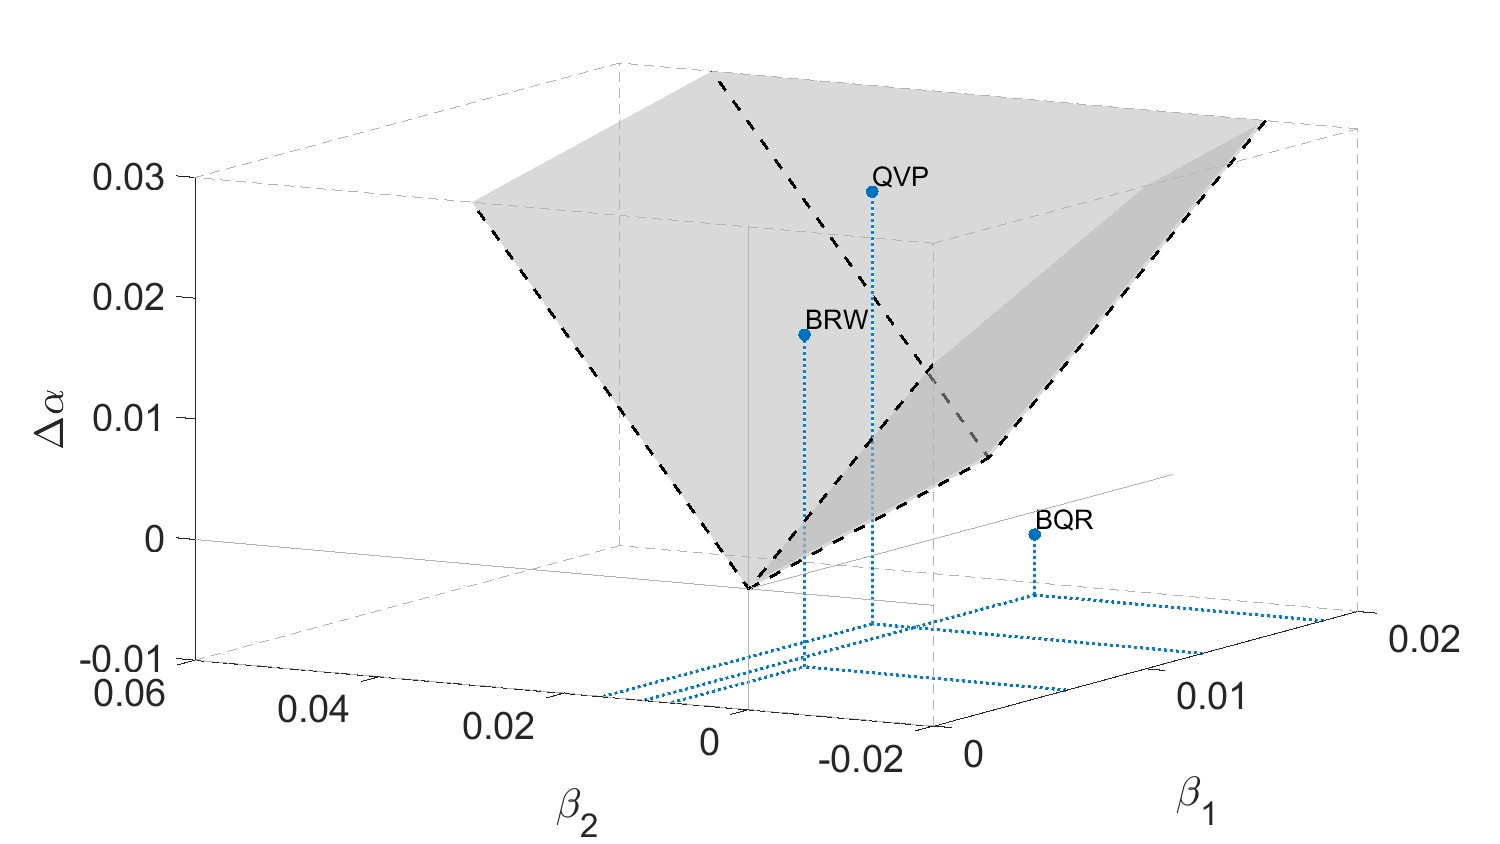
\includegraphics[width=1\textwidth]{Figures/SmallMCFig_3D_Q=2.jpg}
    \end{subfigure}%
    \hfill
    \begin{subfigure}[t]{0.48\textwidth}
        \centering
        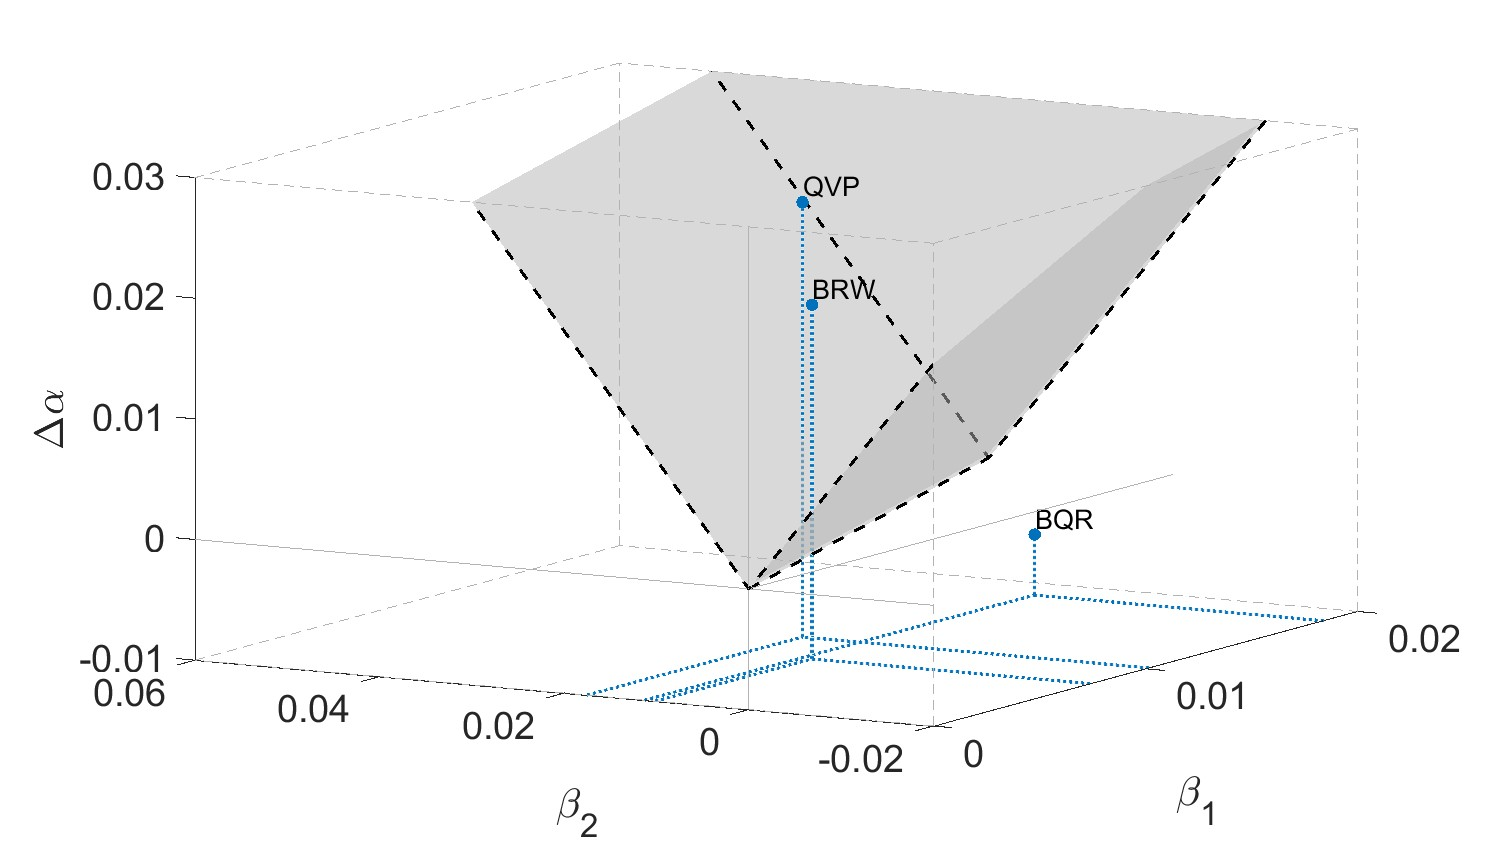
\includegraphics[width=1\textwidth]{Figures/SmallMCFig_3D_Q=20.jpg}
    \end{subfigure}
    \caption{Means of the difference $\Delta\alpha = \alpha_{q}-\alpha_{q-1}$ and $(\beta_{q},\beta_{q-1})$ (blue points) for the $50^{\mathrm{th}}$ and $51^{\mathrm{st}}$ quantiles for the $\mathrm{QVP}$, $\mathrm{BQR}$ and $\mathrm{BRW}$ models. The grey area is the space in which the quantile curves are non-crossing. In the left figure, $\mathcal{Q}=2$, and in the right $\mathcal{Q}=20$ (19 equidistant quantiles and the $51^{\mathrm{st}}$ quantile).}
    \label{fig:nc-zone}
\end{figure}
To visually motivate that this is the case, we plot in Figure~\ref{fig:nc-zone}, the posterior means of the proposed $\mathrm{QVP}$ along-side  the $\mathrm{BQR}$ model with uninformative priors which estimates quantiles independently, as well as the frequentist model of \citet{bondell2010noncrossing}, $\mathrm{BRW}$. The grey area which indicates the space for which two adjacent quantile regression functions are non-crossing. We estimate the models for the median and $51^{\mathrm{st}}$ quantile. While the $\mathrm{BQR}$ leads to posterior point-estimates outside the space of non-crossing, the penalisation implied by the $\mathrm{QVP}$%\footnote{\tibi{The QVP prior used for this figure was constructed in such a way that the $\Delta\alpha$ is ignored, i.e. the Lagrangian is on the differences on the $\beta$ coefficients. This does not change the overall behaviour as can be seen in the figure: the shrinkage with quantile specific tuning parameters yields $\beta$ estimates in the non-crossing volume. The appendix contains further Monte Carlo results showing that the performance of the proposed QVP prior, and the QVP prior with $\Delta\alpha$ influencing the shrinkage parameter yield similar results}}
, and naturally the $\mathrm{BRW}$ model, lead  to coefficient estimates inside the non-crossing area. It would be expected that as quantiles are chosen to be further apart ($\Delta\alpha$ increases, volume of grey area increases), one would obtain estimates of all models in the non-crossing area. However, when the modeller wants to  get an accurate a picture of coefficient-heterogeneity across quantiles, many quantiles are typically estimated which reduces a given pair of quantiles $\Delta\alpha$, thus decreasing the space in the parameter domain for which the quantile curves are non-crossing. We will show that the proposed $\mathrm{QVP}$ scales well with the amount of estimated quantiles.
%
\subsection{Likelihood}\label{sec:likelihood}

%\citet{bondell2010noncrossing} suggest the following non-crossing constraints as a way to improve the %performance of joint quantile estimation:
%%
%%\begin{equation} \label{eq:NC}
%%\begin{split}
    %x_t^T\beta_{\tau_p}&\geq x_t^T\beta_{\tau_{p-1}}%\\
%    x_t^T(\beta_{\tau_p} - \beta_{\tau_{p-1}}) &\geq %0
%%\end{split}
%%\end{equation}
%%
%The above formulation is conceptually simple, but requires $T \times (Q-1)$ constraints to ensure non-crossing. \citet{bondell2010noncrossing} propose using a common evaluation point (called the worst-case scenario), $x_{WC}^T$, as a way to reduce the number of imposed constraints to $(Q-1)$.\footnote{A further requirement to obtain non-crossing constraints of \citet{bondell2010noncrossing} is to decompose $(\beta_{k,\tau_p}-\beta_{k,\tau_{p-1}})=(\gamma_{k,\tau_p}^+-\gamma_{k,\tau_p}^-)$, where both $\gamma_{k,\tau_p}^i\geq0$.} This makes estimation feasible. \citet{bondell2010noncrossing} propose setting show that imposing such constraints leads to improvements %in quantile regression estimates.
%%
%Equation (\ref{eq:NC}) makes it clear that one needs to impose structure on the difference (across quantiles) in coefficients, $\gamma_{\tau_p}=\beta_{\tau_p} - \beta_{\tau_{p-1}}$. \citet{szendrei2023fused} show the direct link between the non-crossing constrain and fused-shrinkage and non-crossing quantiles, which we summarise in the %following theorem:
%\tibi{things: 1) define $\xi \tau_q$, 2) $\alpha$, 3) quick mention that one can split the difference %into + and - differences}
%%%
%%\begin{theorem} \label{theorem:NC=FLASSO}
    %In the Fused LASSO of \citet%{jiang2013interquantile},
%%\begin{equation}
    %%\begin{split}
        %\hat{\beta}_{JWB}&=\underset{\beta}{argmin}\sum^{Q}_{q=1}\sum^{T}_{t=1}\rho_{\tau_q}(y_{t}%-x_t^T\beta_{\tau_q}-\xi{\tau_q})\\
%        &s.t.~k_{\tau_q}^* \geq \sum^K_{k=1}(\gamma_%{k,\tau_q}^++\gamma_{k,\tau_q}^-),
    %%\end{split}
%%\end{equation}
%non-crossing constraints are equivalent to Fused LASSO shrinkage when $k_{\tau_q}\propto \frac{\gamma_%{0,\tau_q}}{\alpha}$.
    %%Non-crossing constraints are a type of Fused $\ell_1$ shrinkage with quantile specific tuning parameter. This quantile specific tuning paramter is determined by the $\gamma_{0,\tau_q}$ and $\alpha$ terms, with the combination of these regulating the degree of quantile %variation.
%%\end{theorem}
%%
%%\begin{proof}
    %Please see \citet{szendrei2023fused} for the %proof.
%%\end{proof}
%%
%While, \citet{szendrei2023fused} propose a set of adaptive non-crossing constraints to tackle non-crossing, their key message of quantile specific shrinkage is amenable to Bayesian estimation. To this end, we develop a quantile varying parameter Bayesian framework where we shrink the difference in %%the coefficients.
%
%%Consider a vector of parameters $\beta \in \mathbb%{R}%^K$ and the objective is to minimise some exp%ected %loss function for data, $x$:
%%
%%\begin{equation} \label{eq:QR_Bissiri}
%    L(\beta)=\int l(\beta,x)dF_0(x),
%\end{equation}
%%
%where $F_0()$ is some unknown distribution function from which iid observations of $x$ arise. 

%
Let $\vartheta$ contain parameters: $\{\alpha_q,\beta_0,\beta_q\}$. Assume prior beliefs about $\vartheta$ are represented by $p(\vartheta)$, then a valid and coherent update of $p(\vartheta)$, following the general belief updating framework of \citet{bissiri2016general}, is to the posterior $p(\vartheta|X)$:
%
\begin{equation}
    p(\vartheta|X)\propto \exp\left(-\ell\left(\vartheta,x\right)\right)p(\vartheta),
\end{equation}
%
where $\ell\left(\vartheta,X\right)=\sum_{q=1}^{\mathcal{Q}}\sum_{t=1}^{\mathcal{T}} \rho_{\tau_q} \left( y_t - \alpha_q - x_t^T\beta_0 - x_t^T\beta_q\right)$.\footnote{The general updating of beliefs framework of \citet{bissiri2016general} includes an unknown scalar multiplying the loss function in order to calibrate the amount of relative information from the data vis-a-vis the prior. We follow the recommendations of Bayesian quantile literature \citep{yu2001bayesian,li2010bayesian} to assume that this scale is equal to 1. \citet{mclatchie2025predictive} show that large enough data, the scale only marginally influences inference.} Exponentiation of the loss function is equivalent up to a constant of proportionality to the commonly employed asymmetric-Laplace ($\mathcal{ALD}$) working likelihood used for probabilistic quantile regression modelling:
%
\begin{IEEEeqnarray}{rl}
    l\left(\vartheta,X\right) &\;= \exp\left(-\sum^{\mathcal{Q}}_{q=1}\sum^{\mathcal{T}}_{t=1}\rho_{\tau_q}(y_t- \alpha_q -x_t^T\beta_0 -x_t^T\beta_{q})\right) \\
    & \; \propto \prod_{q=1}^\mathcal{Q} \prod_{t=1}^T \mathcal{ALD}\left(y_t\vert\alpha_q,\beta_0,\beta_q,x_t\right) \\
    & \; = \left( \prod_{q=1}^{\mathcal{Q}}\prod_{t=1}^{\mathcal{T}} \tau_q(1-\tau_q) \right) \exp\left(-\sum_{q=1}^{%\mathcal{T}
    \mathcal{Q}}\sum_{t=1}^{\mathcal{T}} \rho_{\tau_q}\left(y_t - \alpha_q -x_t^T\beta_0 -x_t^T\beta_q\right)\right).
\end{IEEEeqnarray}
Hence, minimising the expected multiple quantile loss is equivalent to maximising the combination of the individual $\mathcal{ALD}$ likelihoods of each quantile, where quantiles are assumed to be exchangeable, conditional on $\left(\alpha_q,\beta_0,\beta_q\right)$. For computational convenience, we make use of the fact that the $\mathcal{ALD}$ can be written as a mixture of normal distributions, with the scale parameter having an exponential distribution, following \citet{kozumi2011gibbs}:
%
\begin{equation}
    \begin{split} 
    l\left(\vartheta,X\right) & \propto \int_0^{\infty} \frac{1}{\sqrt{2\zeta_q^2\omega_q}} \exp\left(-\sum_{q=1}^{\mathcal{Q}}\sum_{t=1}^{\mathcal{T}}(y_t - \alpha_q- x_t^T\beta_0 -x_{t}^T\beta_q - \theta_q \omega_{q,t})^2/(2\omega_{q,t}\zeta_q^2)\right) \\
    &  \times \prod_{t=1}^{\mathcal{T}} \mathrm{e}^{\omega_{i,t} } d\omega_{i,t}, \quad \forall i \in \{1,\dots,\mathcal{Q}\},\; \forall t \in {1,\dotsc,\mathcal{T}} \\ 
    \end{split}
\end{equation}
%
where $\theta_q = (1-2\tau_q)/(\tau_q(1-\tau_q))$, $\zeta_q^2 = 2/(\tau_q(1-\tau_q))$, and $\omega_{q,t}\sim \mathrm{exp}\left(\sigma^{y}_q\right)$. 
To vectorise across $q$, define $\boldsymbol{y} = \mathbbm{1}_{\mathcal{Q}} \otimes y$, $\boldsymbol{X} = \mathbbm{I}_{\mathcal{Q}} \otimes  X$, where $\mathbbm{1}_{\mathcal{Q}}$ denotes a $\mathcal{Q}$-dimensional vector of ones, and let $\mathbbm{I}_Q$ be the identity matrix of dimension $Q\times Q$. Further, we denote the location adjustment due to data augementation by $\mu_{q,t} = \theta_q\omega_{q,t}$ . Denote $\omega_q = (\omega_{q,1},\dotsc,\omega_{q,\mathcal{T}})^T$, $\boldsymbol{\alpha} = (\alpha_1,\dotsc,\alpha_1,\dotsc,\alpha_\mathcal{Q},\dotsc,\alpha_\mathcal{Q}) \in \mathbbm{R}^{\mathcal{Q} \mathcal{T}}$, $\boldsymbol{\mu} = (\mu_{1,1},\dotsc,\mu_{1,\mathcal{T}},\dotsc,\mu_{\mathcal{Q},1},\dotsc,\mu_{\mathcal{Q},\mathcal{T}})^T$, then the joint likelihood implied is:
%
\begin{equation} \label{eq:integrated_likelihood}
 \boldsymbol{y}  \sim \int_{0}^{\infty} \mvn\left( \boldsymbol{\alpha} + \boldsymbol{X} \left(\mathbbm{1}_{\mathcal{Q}} \otimes \beta_0\right) +  \boldsymbol{X}\boldsymbol{\beta} + \boldsymbol{\mu}, \boldsymbol{\Omega}\right) \times e^{−\boldsymbol{\omega} } d\boldsymbol{\omega},
\end{equation}
%
where $\boldsymbol{\beta} = (\beta_1^T,\dotsc,\beta_{\mathcal{Q}}^T)^T$ captures the heterogeneity induced by the covariates, and $\boldsymbol{\Omega} =\text{diag}(\omega_1,\dotsc,\omega_{\mathcal{Q}})$.  $\mvn()$ stands for the multivariate normal distribution. 
%
\subsection{The QVP Prior}\label{sec:qvp-prior}
%
Consider again the penalised quantile objective of Equation~\ref{eq:fused-objective-function}. A probabilistic generalisation can be found by the following discrete state space representation: %Section \dk{Reference to likelihood section} motivates a particular view onto the estimation problem where information between parameters are shared among quantiles. In particular consider the following model\dk{make explicit that estimating composite vector as the starting condition is equivalent to intialising the state space at that vector}:
%
\begin{IEEEeqnarray}{rl}
     y_{t} & = \alpha_q + x_t^{T}\beta_q + \mu_{q,t} + \epsilon_{q,t}^y,\; \epsilon^y_{q,t}\sim\normal\left(0,\theta_q^2\sigma^y_q\omega_{q,t}\right), \; t = 1,\dotsc, \mathcal{T} \label{eq:observation-equation-centred} \\
     \beta_q & = \beta_{q-1} + \epsilon^{\beta}_q,\; \epsilon^{\beta}_q \sim \mvn\left(0,\Sigma_{q}\right),  \; q  = 1,\dotsc,\mathcal{Q} \label{eq:state-equation-centred} \\
     \beta_0 & \sim \mvn\left(0,\Sigma_0\right) \label{eq:starting-condition-cented}, \; \alpha \propto \mathbbm{1}_{Q\mathcal{T}},
\end{IEEEeqnarray}
%
where $\beta_0$ is the quantile invariant vector and $\Sigma_q = \text{diag}(\sigma_{q,1}^2,\dotsc,\sigma_{q,K}^2)$. $\Sigma_q$ controls the variability of the coefficients between quantiles and therefore how strongly correlated the coefficients are.\footnote{Allowing for non-zero off diagonals would allow for any quantile  coefficient to affect any of the other estimated quantiles directly. While relevant, we leave investigation of the properties of this modelling approach to future research.} Modelling $\epsilon_q^{\beta}$  with Laplacian densities would create the exact Bayesian equivalent to the penalisation implied by the lasso penalty in the objective function. Namely, when $\beta_q - \beta_{q-1} \sim \mathcal{MAL}\left(0, \Sigma_q  \right)$, or equivilantly, $\beta_q \sim \mathcal{MAL}\left(\beta_{q-1}, \Sigma_q  \right)$, where $\mathcal{MAL}\left( \right)$ stands for the multivariate Laplace distribution \citep{kotz2001asymmetric}. A similar logic is presented in the derivation of the univariate lasso prior of \citep{park2008bayesian}. We, however, follow the more recent literature on shrinkage priors that show superior shrinkage properties with normal kernels \citep{carvalho_handling_2009,piironen_hyperprior_2017}. To adhere to the convention of the state-space literature, we will refer to Equation~\ref{eq:observation-equation-centred} as the observation equation, and Equation~\ref{eq:state-equation-centred} as the state equation for quantile $\tau_q$ respectively.
%

The state vector $\beta_0$ plays a special role in this model setup. It is both the initialisation of the state process, and equivalent to the quantile invariant vector in Objective~\ref{eq:fused-objective-function}. This can be easily verified by backward substitution of the state equation into the observation equation. In fact, when $\mathbf{\beta}=\boldsymbol{0}$, then $\beta_0$ is equivalent to the composite quantile regression vector, considered in \citet{zou2008composite}. The significance of this for the shrinkage properties will be further investigated in Section~\ref{sec:theoretical-properties}.
%

The state-space representation results in a particular structure to the joint prior. Write the state process in Equation~$\ref{eq:state-equation-centred}$ stacked across $\mathcal{Q}$ in matrix form as:
%
\begin{equation}
    H\boldsymbol{\beta} = \tilde{\boldsymbol{\beta}} + \boldsymbol{\epsilon^{\beta}},
\end{equation}
%
where $\boldsymbol{\epsilon^{\beta}} \sim \mvn(0,\boldsymbol{\Sigma})$, $\boldsymbol{\Sigma} = \mathrm{diag}(\Sigma_1,\dotsc,\Sigma_{\mathcal{Q}})$, $\boldsymbol{\tilde{\beta}} = (\beta_0^T,0,\dotsc,0)^T$ and
%
\begin{equation}
    \boldsymbol{H} = 
    \begin{pmatrix}
        \mathbbm{I}_{K} & 0 & 0 & \dotsc & 0 \\ 
        -\mathbbm{I}_{K} & \mathbbm{I}_{K} & 0 & \dotsc & 0 \\ 
        0 & -\mathbbm{I}_{K} & \mathbbm{I}_{K} & \dotsc & 0 \\
        \vdots &  & \ddots & \ddots & \vdots \\
        0 & 0 & \dotsc & -\mathbbm{I}_{K} & \mathbbm{I}_{K} \\
    \end{pmatrix}.
\end{equation}
%
$\boldsymbol{H}$ is a $\mathcal{Q}K \times \mathcal{Q}K$ difference matrix, which is invertible since $|\boldsymbol{H}| = 1$. It is straightforward to show that $\boldsymbol{H}^{-1}\boldsymbol{\tilde{\beta}} = \mathbbm{1}_{\mathcal{Q}} \otimes \beta_0$. Then, the joint prior for $\boldsymbol{\beta}$, conditional on $\left(\beta_0,\boldsymbol{\Sigma}\right)$ is
%
\begin{equation}
    (\boldsymbol{\beta}\mid \beta_0,\boldsymbol{\Sigma}) \sim \mvn\left(\mathbbm{1}_{\mathcal{Q}} \otimes \beta_0,(\boldsymbol{H}^T\boldsymbol{\Sigma}^{-1}\boldsymbol{H})^{-1}\right),
\end{equation}
%
Due to the close connection to joints priors for time-varying parameter regression models in which $\beta$ is indexed by time, we call this prior the joint quantile-varying parameter ($\QVP$) prior.
%
And by standard manipulations, the posterior is given by
%
\begin{equation} \label{eq:Posterior_beta_centred}
    \left(\boldsymbol{\beta} \mid \boldsymbol{y},\dotsc\right) \propto \mvn\left(\overline{\boldsymbol{\beta}}, \boldsymbol{\text{K}_{\beta}}^{-1}\right),
\end{equation}
%
where
%
\begin{equation}
    \begin{split}
        \boldsymbol{\text{K}_{\beta}} & = \boldsymbol{H}^T\boldsymbol{\Sigma}^{-1}\boldsymbol{H} + \boldsymbol{X}^T\boldsymbol{\Omega}^{-1}\boldsymbol{X} \\
        \overline{\boldsymbol{\beta}} & = \boldsymbol{\text{K}_{\beta}}^{-1} \left(\boldsymbol{H}^T\boldsymbol{\Sigma}^{-1}\boldsymbol{H}\left(\mathbbm{1}_{\mathcal{Q}} \otimes \beta_0\right) + \boldsymbol{X}^T\boldsymbol{\Omega}^{-1}\boldsymbol{y^{*}}\right), 
    \end{split}
\end{equation}
and $\boldsymbol{y^{*}}  =  \boldsymbol{y} - \boldsymbol{\alpha} - \boldsymbol{\mu}$.
%
\subsection{Fused Horseshoe Prior}
%
The priors on $\boldsymbol{\Sigma}$ determine the amount of quantile variation. We model explicitly: 1) adaptivity of shrinkage on the difference in coefficients across quantiles, specific to each covariate, 2) global regularisation of each $\beta_q-\beta_{q-1}$~difference vector. Therefore, it is natural to follow the global-local prior literature where the prior hierarchy on $\sigma_{q,j}$ employs a mixture of fat-tailed distributions with singularity at 0 to allow for both large and small changes in coefficients. A plethora of priors can be considered \citep{polson_half-cauchy_2012}, however, we consider here the horseshoe prior \citep{carvalho_handling_2009}, adapted to fused shrinkage. In particular, define $\sigma^2_{q,j} = \nu_q^2\lambda_{q,j}^2$,\footnote{Setting double-Laplace priors for $\lambda_{q,j}$, the exact Bayesian interpretation of the absolute deviation penalisation of the motivating objective function in Equation~\ref{eq:motivating-obj} can be recovered.} then the fused horseshoe prior is
%
\begin{equation}\label{eq:prior-differences-centred}
    \nu_q\sim C_{+}\left(0,1/\sqrt{\mathcal{T}}\right),\quad \lambda_{q,j}\sim C_{+}(0,1),
\end{equation}
%
where $C_+()$ stands for the half Cauchy distribution. Following \citet{piironen_hyperprior_2017}, we scale the global parameter by the number of data points. While $\nu_q$ controls overall approximate sparsity of differences in quantiles, the local scales $\lambda_{q,j}$ control the local adaptivity in how much the differences are shrunk dependent on the quantile level as well as the covariate.
%
\subsection{Prior on $\beta_0$}
%
We again set a horseshoe prior. Let $\Sigma_0 = \nu^2_0\text{diag}(\lambda^2_{0,1},\dotsc,\lambda^2_{0,K})$, then
%
\begin{equation} \label{eq:prior_level}
\begin{split}
    \beta_0 & \sim \mvn\left(0,\Sigma_0\right) \\
    \pi\left(\nu_0\right) & \sim C_{+}\left(0,1/\sqrt{\mathcal{T}\mathcal{Q}}\right),\quad \pi\left(\lambda_{0,j}\right) \sim C_{+}\left(0,1\right). 
\end{split}
\end{equation}
%
This prior may also induce approximate sparsity in the quantile invariant vector.
%

We summarise the $\QVP$ prior model with the following definition:
\begin{definition}\label{def:qvp_centred}
The $\QVP$ prior defined over $\mathcal{Q}$ quantiles with quantile-adaptive horseshoe  regularisation yields the following model structure, where $q = 1,\dotsc,\mathcal{Q}$ and $j = 1,\dotsc,K$:
    %
    \begin{IEEEeqnarray}{rl}
        \boldsymbol{y} \;& \sim\mvn\left(\boldsymbol{\alpha} + \boldsymbol{\mu} + \boldsymbol{X}\boldsymbol{\beta},\boldsymbol{\Omega}\right)\label{eq:qvp_likelihood} \\
        \boldsymbol{\beta} \;&\sim \mvn\left(\mathbbm{1}_{\mathcal{Q}}\otimes\beta_0, \left(\boldsymbol{H}^T\boldsymbol{\Sigma}^{-1}\boldsymbol{H}\right)^{-1}\right)\label{eq:qvp_beta_prior} \\
                \beta_0 \;&\sim \mvn\left(0, \Sigma_0\right)\label{eq:qvp_beta_0_prior} \\
        \boldsymbol{\Sigma}\;&=\mathrm{diag}\left(\sigma^2_{1,1},\dotsc,\sigma^2_{1,K},\dotsc,\sigma^2_{\mathcal{Q},1},\dotsc,\sigma^2_{\mathcal{Q},K}\right),\; \sigma^2_{q,j} = \nu_q^2\lambda^2_{q,j} \\
        \Sigma_{0}\;&=\mathrm{diag}\left(\sigma^2_{0,1},\dotsc,\sigma^2_{0,K}\right),\; \sigma^2_{0,j} = \nu_0^2\lambda^2_{0,j} \\
        \nu_q\;& \sim C_+\left(0,\frac{1}{\sqrt{\mathcal{T}}}\right),\;        \lambda_{q,j}\;\sim C_+\left(0,1\right),\; \nu_0 \sim C_{+}\left(0,\frac{1}{\sqrt{\mathcal{T}\mathcal{Q}}}\right) \\
        \mu_{q,t}\;&= \theta_q\omega_{q,t},\;\omega_{q,t}\sim \mathrm{exp}\left(\sigma^{y}_q\right) \\
        \boldsymbol{\alpha}\;&\propto\mathbbm{1}_{\mathcal{Q}\mathcal{T}} \\
        \sigma^y_q\;&\sim p\left(\right),
    \end{IEEEeqnarray}
    %
\end{definition}
%
where $p()$ stands for some probability density. With uninformative priors $\boldsymbol{\alpha} \propto 1$,
 any location shift in the quantile function of $\boldsymbol{\beta}$ is determined by the data only. Notice, that this deviates from incrementing the posterior with the difference prior on $alpha_q-\alpha_{q-1}$ in \ref{eq:fused-objective-function}, which would influence only the conditional posterior of the quantile specific global-shrinkage. For this and the additional reason that shrinking toward the quantile invariant vector favours shrinking toward parallel quantile curves, we opt for uninformative priors. However for completeness, we present simulation evidence in Appendix~\ref{subsubsec:alpha-predictions} with the full difference prior on $\alpha_q-\alpha_{q-1}$. The results are virtually identical. Finally, we set the relatively uninformative prior of $\sigma^y_q \sim \IG{0.1,0.1}$, where $\IG{\underline{a},\underline{b}}$ stands for the inverse-Gamma distribution with rate $\underline{a}$ and scale $\underline{b}$. 
%